\begin{enumerate}

          \textbf{NOTE:  YOU MUST HAVE PYTHON3 ENABLED IN ORDER TO RUN THE QUERYING SCRIPT. PLEASE TYPE THE FOLLOWING COMMAND:}
                \begin{verbatim}
                source /opt/rh/python33/enable
                \end{verbatim}
    \item Step by step running
        \begin{itemize}
            \item Open up a terminal in Linux with the project downloaded.
            \item Change your working directory to \begin{verbatim}/mapreduce/ \end{verbatim}
            \item Type the following command: \begin{verbatim} ./execute.sh <list of files to run on> \end{verbatim}
            \item After MapReduce finishes, the querying script will run. You can now enter in a specific word or list of words to search for. (See the following section for screenshots of code working and example use cases.)
           \end{itemize}
    \item screenshot of run command \\
    
\begin{figure}[!htbp] 
 \frame{ 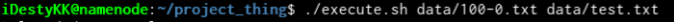
\includegraphics[width=\textwidth]{hadoop_run.PNG}}
  \caption{An example of the run script.}
\end{figure}

\end{enumerate}